\documentclass[dvipsnames,border=3pt]{standalone}
\usepackage{tikz}
\usetikzlibrary{arrows}
\usetikzlibrary{shapes}
\usepackage{enumitem}
\usepackage{bm}
\usepackage{mathdots}
\usepackage{amsmath}
\usetikzlibrary{shadings}
\usetikzlibrary{decorations.pathreplacing}
\usepackage{helvet}
\usetikzlibrary{arrows.meta}
\usepackage{graphicx}
\usepackage{pgfplots}
\usepackage{pgfplotstable}
\usepackage{filecontents}
\usetikzlibrary{plotmarks}
\pgfplotsset{compat=newest}

\renewcommand{\familydefault}{\sfdefault}

\definecolor{mylightgray}{cmyk}{0,0,0,0.1}
\definecolor{mypurple}{HTML}{6E016B}
\usetikzlibrary{arrows,decorations.pathmorphing,backgrounds,fit,positioning,shapes.symbols,chains}

\begin{document}

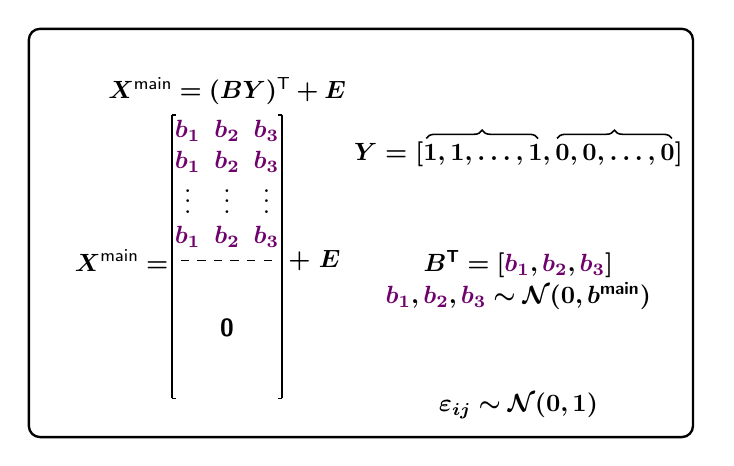
\begin{tikzpicture}
    % trim=left botm right top
    
    \node[draw, rounded corners=4, line width=0.3mm, text width=8.2cm, text height=4.95cm] at (-0.3,0) {};
    %\node[circle,draw,line width=0.2mm,xscale=1.2,yscale=1.2,fill=GreenYellow] at (-3.82,1.64) {};
    %\node at (-3.82,1.64) {\textbf{5}};
    
    %\node[draw,rounded corners=2,line width=0.2mm,fill=gray!50,text height=0.35cm, text width=4.1cm,shading angle=45] at (0,1.58) {}; % random graph
    %\node[xscale=1.1,yscale=1.1] at (0,1.56) {\textbf{Main Effect Simulation}}; 
    
    \node[xscale=0.9,yscale=0.9] at (-2,1.8) {\bm{$X^\text{main} = (B Y)^\text{T} + E$}};
    
    \node[xscale=0.9,yscale=0.9] at (-3.34,-0.35) {\bm{$X^\text{main} =$}};
    \node[xscale=0.9,yscale=0.9] at (-0.89,-0.35) {\bm{$+$} \bm{$E$}};
    
    % row 1
    \node[xscale=0.9,yscale=0.9] at (-2.5,1.3) {\textcolor{mypurple}{\bm{$b_1$}}};
    \node[xscale=0.9,yscale=0.9] at (-2,1.3) {\textcolor{mypurple}{\bm{$b_2$}}};
    \node[xscale=0.9,yscale=0.9] at (-1.5,1.3) {\textcolor{mypurple}{\bm{$b_3$}}};
    
    % row 2
    \node[xscale=0.9,yscale=0.9] at (-2.5,0.9) {\textcolor{mypurple}{\bm{$b_1$}}};
    \node[xscale=0.9,yscale=0.9] at (-2,0.9) {\textcolor{mypurple}{\bm{$b_2$}}};
    \node[xscale=0.9,yscale=0.9] at (-1.5,0.9) {\textcolor{mypurple}{\bm{$b_3$}}};
    
    % row 3 (dots)
    \node[xscale=0.95,yscale=0.95] at (-2.5,0.5) {$\vdots$};
    \node[xscale=0.95,yscale=0.95] at (-2,0.5) {$\vdots$};
    \node[xscale=0.95,yscale=0.95] at (-1.5,0.5) {$\vdots$};
    
    % row 4
    \node[xscale=0.9,yscale=0.9] at (-2.5,-0.05) {\textcolor{mypurple}{\bm{$b_1$}}};
    \node[xscale=0.9,yscale=0.9] at (-2,-0.05) {\textcolor{mypurple}{\bm{$b_2$}}};
    \node[xscale=0.9,yscale=0.9] at (-1.5,-0.05) {\textcolor{mypurple}{\bm{$b_3$}}};
    
    % dashed dividing line
    \draw[line width=0.2mm,dashed] (-2.59,-0.35) -- (-1.35,-0.35);
    
    % zero in lower block
    \node[xscale=0.9,yscale=0.9] at (-2,-1.2) {\textbf{0}};
    
    % left bracket
    \draw[line width=0.2mm] (-2.7,-2.1) -- (-2.7,1.5);
    \draw[line width=0.2mm] (-2.7,-2.1) -- (-2.65,-2.1);
    \draw[line width=0.2mm] (-2.7,1.5) -- (-2.65,1.5);
    
    % right bracket
    \draw[line width=0.2mm] (-1.3,-2.1) -- (-1.3,1.5);
    \draw[line width=0.2mm] (-1.3,-2.1) -- (-1.35,-2.1);
    \draw[line width=0.2mm] (-1.3,1.5) -- (-1.35,1.5);
    
    % outcome vector
    \node[xscale=0.9,yscale=0.9] at (1.7,1) {$\boldsymbol{Y = [1, 1, \dots, 1, 0, 0, \dots, 0]}$};
    
    % effect size vector
    \node[xscale=0.9,yscale=0.9] at (1.7,-0.4) {\bm{$B^\textbf{T} = [\textcolor{mypurple}{b_1}, \textcolor{mypurple}{b_2}, \textcolor{mypurple}{b_3}]$}};
    \node[xscale=0.9,yscale=0.9] at (1.7,-0.8) {\bm{$\textcolor{mypurple}{b_1},\textcolor{mypurple}{b_2},\textcolor{mypurple}{b_3} \sim \mathcal{N}(0,b^\textbf{main})$}};
    
    % gaussian error
    \node[xscale=0.9,yscale=0.9] at (1.7,-2.2) {\bm{$\varepsilon_{ij} \sim \mathcal{N}(0,1)$}};
    
    \draw [decorate,decoration={brace,amplitude=3pt,aspect=0.5},line width=0.2mm,draw] (0.53,1.2) -- (1.95,1.2) node [black,xshift=9pt] {\footnotesize};
    \draw [decorate,decoration={brace,amplitude=3pt,aspect=0.5},line width=0.2mm,draw] (2.19,1.2) -- (3.65,1.2) node [black,xshift=9pt] {\footnotesize};
    
\end{tikzpicture}
    
\end{document}